\documentclass[12pt]{article}
\usepackage[utf8]{inputenc}
\usepackage{mathtools}
\usepackage{pdfpages}
\usepackage{amssymb}

\title{Robot Programming Methods}
\author{Krzysztof Rudnicki, 307585}
\date{\today}

\begin{document}

\maketitle
\section{Scenario description}
\begin{itemize}
	\item Conduct scene analysis, identify objects based on specific shapes (triangular, square, or circular), and determine their orientations.
	\item Choose one object from the group.
	\item Create initial grasp positioning, final grasp positioning, and plan the route for reaching the object.
	\item Implement the planned route to reach the object.
	\item Grasp and lift the selected object.
	\item Identify the appropriate mold (either triangular, square, or circular) for the object.
	\item Plan the route towards the identified mold.
	\item Follow the planned route to the mold.
	\item Release the object into the mold.
\end{itemize}
\subsection{Hardware setup}

\begin{center}
\begin{tabular}{ | p{3cm} | p{3cm} | p{3cm} | p{3cm} |}
\hline
Hardware & Task & Degrees of freedom & Role \\ 
 \hline
Manipulator & Approaching and translocating objects & 6 & effector \\
 \hline
Suction gripper & To pick up objects & N/A & effector \\
 \hline
 RGB-D camera (Kinect) & To identify the object and enable its localization in time & N/A & exteroceptor \\

 \hline
\end{tabular}
\end{center}

\subsection{Notation}
\begin{description}
    \item[B] - robot base reference frame
    \item[E] - end-effector frame
    \item[K] - Kinect frame
    \item[M] - Mold frame
    \item[v] - v-th object frame
    \item[c] - current pose
    \item[T] - transformation
    \item[$\prescript{B}{E}{T}$] - Effector with respect to base
   	\item[$\prescript{B}{K}{T}$] - Kinect with respect to base
   	\item[$\prescript{B}{v}{T}$] - v-th object with respect to base
   	\item[$\prescript{B}{M}{T}$] - mold with respect to base
    \item[$\prescript{E}{K}{T}$] - Kinect with respect to effector
   	\item[$\prescript{E}{v}{T}$] - v-th object with respect to effector
   	\item[$\prescript{E}{M}{T}$] - mold with respect to effector
   	\item[$\prescript{K}{v}{T}$] - v-th object with respect to Kinect
    \item[$\prescript{K}{m}{T}$] - mold with respect to Kinect
   	\item[$\prescript{M}{v}{T}$] - v-th object with respect to mold
\end{description}

\section{Internal structure of agents}
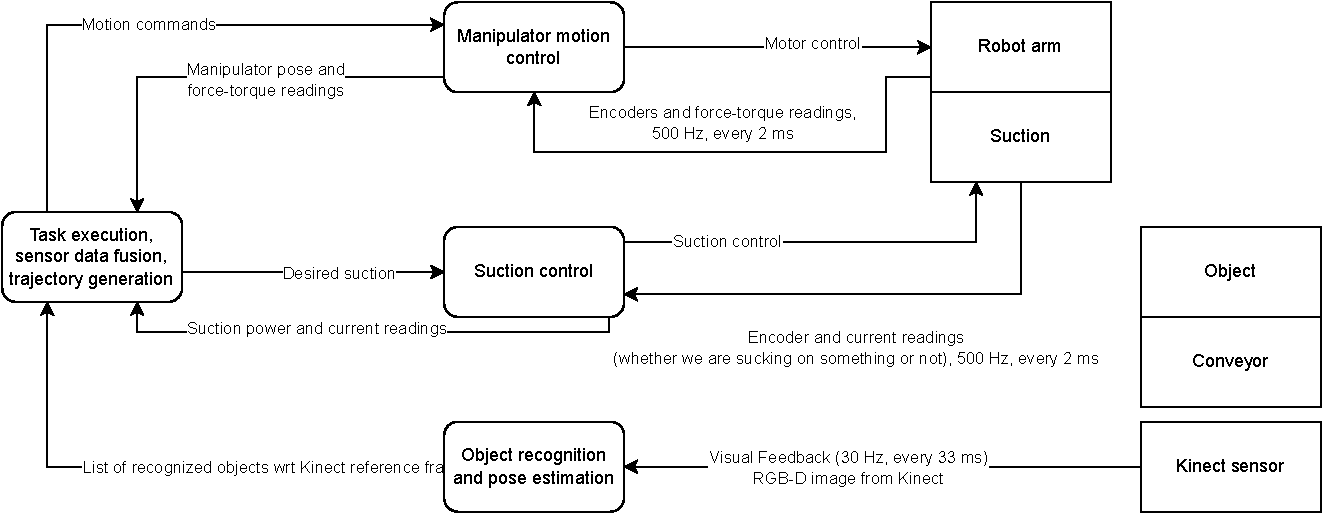
\includepdf[pagecommand=\subsection{General system structure}]{generalSystemStructure.pdf}

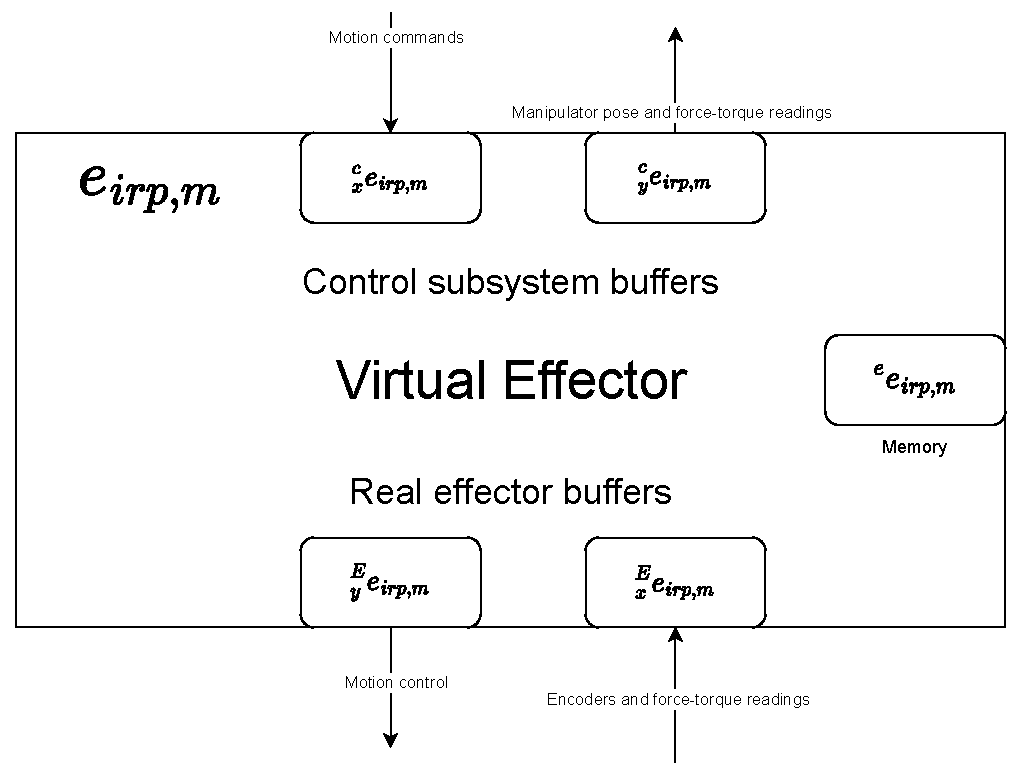
\includepdf[pagecommand=\subsection{Inner structure of the virtual effector}, scale=0.9]{e_irp_m.pdf}

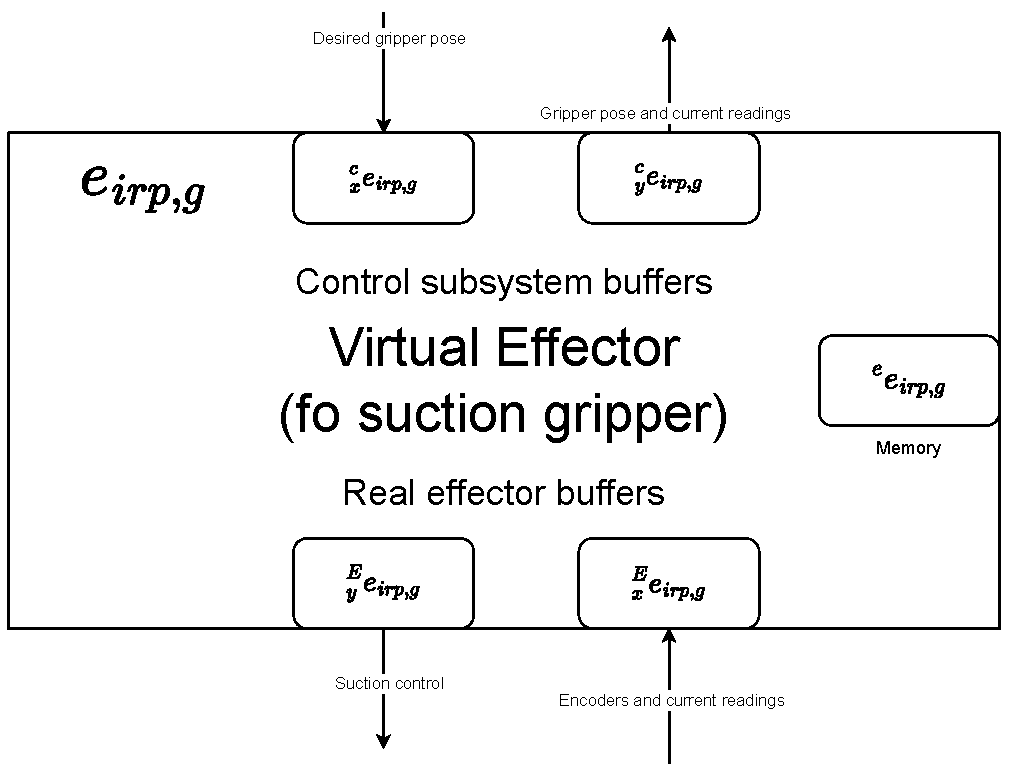
\includepdf[pagecommand=\subsection{Inner structure of the virtual suction gripper effector}, scale=0.9]{e_irp_g.pdf}

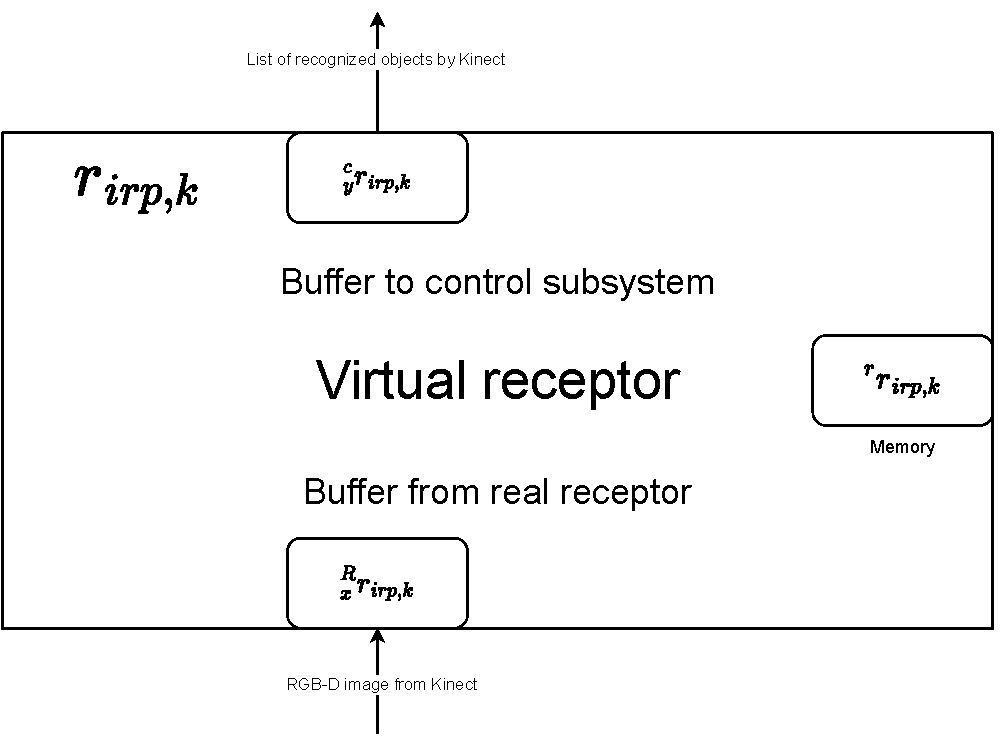
\includepdf[pagecommand=\subsection{Inner structure of the virtual receptor}, scale=0.9]{r_irp_k.pdf}

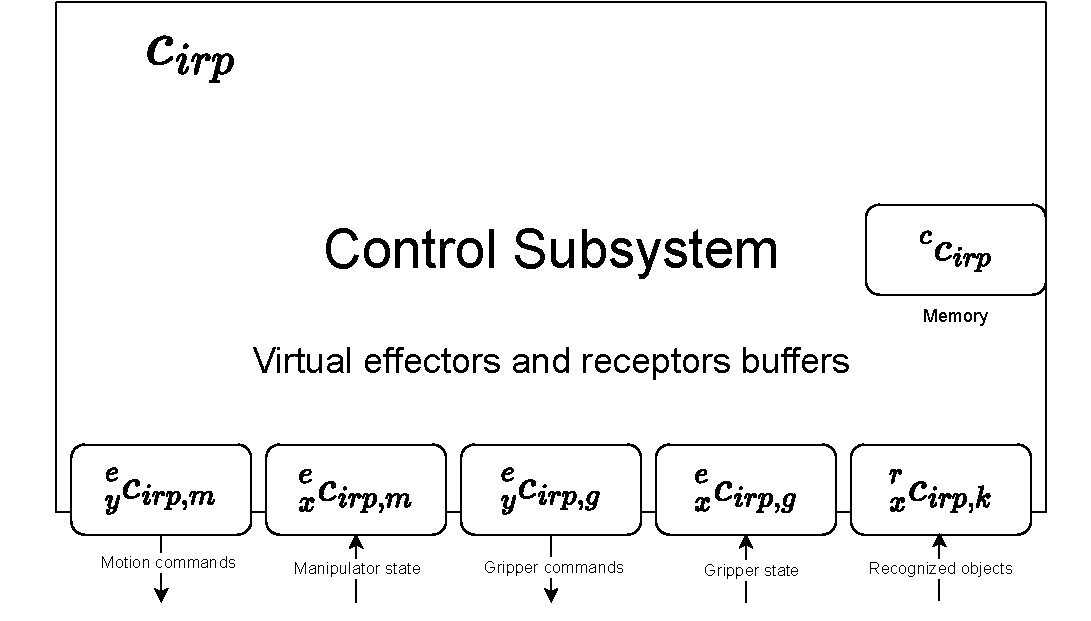
\includepdf[pagecommand=\subsection{Inner structure of the control subsystem}, scale=0.9]{c_irp.pdf}

\section{Sampling rates}
\begin{description}
    \item[$E_{irp, m}$] - 2 miliseconds
	\item[$e_{irp, m}$] - 2 miliseconds
	\item[$E_{irp, g}$] - 2 miliseconds
	\item[$e_{irp, g}$] - 2 miliseconds
	\item[$R_{irp, k}$] - 33 miliseconds
	\item[$r_{irp, k}$] - 33 miliseconds
	\item[$c_{irp}$] - 2 miliseconds (same as fastest virtual effector
\end{description}

\section{General description of virtual effectors/receptors behaviour}
\paragraph{$e_{irp, m}$} - This effector is responsible for maneuvering the arm to align the suction gripper over the targeted item. It communicates the arm's position and the force-torque data to the control subsystem. Once the object is secured, it transports the object to the designated mold, ensuring proper orientation for insertion.

\paragraph{$e_{irp, g}$} - This effector activates the suction when the gripper is accurately positioned. It monitors and conveys the gripper's suction intensity and its grip status to the control subsystem. After the item is secured and positioned over the appropriate mold, this element facilitates the release of the object.

\paragraph{$r_{irp, k}$} - This effector takes care of item identification, determining and communicating their positions to the control subsystem. It also provides details about the rotational adjustments necessary for the picked object, enabling its correct alignment with the mold.

\section{Data Structures (Buffers) of control subsystem}
\subsection{Buffers}
\[ \prescript{r}{x}{c}_{irp, k} = \prescript{c}{y}{r}_{irp, k} \]
\[ \prescript{e}{x}{c}_{irp, g} = \prescript{c}{y}{e}_{irp, g} \]
\[ \prescript{e}{x}{c}_{irp, m} = \prescript{c}{y}{e}_{irp, m} \]
\[ \prescript{e}{y}{c}_{irp, g} = \prescript{c}{x}{e}_{irp, g} \]
\[ \prescript{e}{y}{c}_{irp, m} = \prescript{c}{x}{e}_{irp, m} \]
\subsection{Memory}
\begin{description}
\item[$\prescript{c}{}{c}_{irp}\lbrack\prescript{B}{K}{T}\rbrack$] Kinect sensor pose wrt robot base reference frame
\item[$\prescript{c}{}{c}_{irp} \lbrack \prescript{P}{G}{T} \rbrack $] Transformation between the suction and pre suction poses
\item[$\prescript{c}{}{c}_{irp} \lbrack \prescript{B}{1 \dots V}{O}_c \rbrack $] List of verified object and their types (square, circular or triangular)
\item[$\prescript{c}{}{c}_{irp} \lbrack \prescript{B}{E_g}{T}_d \rbrack $] Suction pose, when the contact with the object is expected
\item[$\prescript{c}{}{c}_{irp} \lbrack \prescript{B}{E_p}{T}_p \rbrack $] Pre-suction pose, where should the final grasp approach begin
\item[$\prescript{c}{}{c}_{irp} \lbrack d_o \rbrack $] Transformation between the suction and pre suction poses
\item[$\prescript{c}{}{c}_{irp} \lbrack \prescript{B}{E_s}{T}_d \rbrack $] Start pose of the manipulator
\item[$\prescript{c}{}{c}_{irp} \lbrack p_o \rbrack $] Level of pressure in suction when suction is turned off
\item[$\prescript{c}{}{c}_{irp} \lbrack \prescript{E}{F}T \rbrack $] Pose of center of the gripper with respect to end-effector 
\item[$\prescript{c}{}{c}_{irp} \lbrack p_p \rbrack $] Vacuum pressure level indicating that the object got picked up
\item[$\prescript{c}{}{c}_{irp} \lbrack \prescript{}{z}V_d, \prescript{}{z}D_d, \prescript{}{z}I_d \rbrack $] Velocity, damping and inertia values (along the Z axis) when approaching the object for suction
\end{description}

\section{Transition functions and terminal conditions}

	\subsection{States and Behaviours}
		\begin{center}
\begin{tabular}{ | c | c| c |}
\hline
$\prescript{c}{}S_{irp, 1}$ & $\prescript{c}{}{B}_{irp, 1}$ & Move to initial pose \\
\hline
$\prescript{c}{}S_{irp, 2}$ & $\prescript{c}{}{B}_{irp, 2}$ & Recognize objects in the scene \\
\hline
$\prescript{c}{}S_{irp, 3}$ & $\prescript{c}{}{B}_{irp, 3}$ & Generate suction parameters\\
\hline
$\prescript{c}{}S_{irp, 4}$ & $\prescript{c}{}{B}_{irp, 4}$ & Move to presuck pose \\
\hline
$\prescript{c}{}S_{irp, 5}$ & $\prescript{c}{}{B}_{irp, 5}$ & Move to suck pose \\
\hline
$\prescript{c}{}S_{irp, 6}$ & $\prescript{c}{}{B}_{irp, 6}$ & Start sucking \\
\hline
$\prescript{c}{}S_{irp, 7}$ & $\prescript{c}{}{B}_{irp, 4}$ & Move to presuck pose \\
\hline
$\prescript{c}{}S_{irp, 8}$ & $\prescript{c}{}{B}_{irp, 7}$ & Move to the molt pose\\
\hline
$\prescript{c}{}S_{irp, 9}$ & $\prescript{c}{}{B}_{irp, 8}$ & Turn off sucking \\
\hline

\end{tabular}
\end{center}
	\subsection{Terminal conditions}
\begin{align}
    \prescript{c}{}{f}_{irp, 1}^{\tau} & \triangleq (\prescript{B}{E}{T}_c = \prescript{B}{E_s}T_d) \\
    \prescript{c}{}{f}_{irp, 2}^{\tau} & \triangleq \prescript{c}{}c_{irp}\lbrack \prescript{B}{1 \dots V}{O}_c \rbrack \rbrack \neq NIL \\
    \prescript{c}{}{f}_{irp, 3}^{\tau} & \triangleq TRUE \\
    \prescript{c}{}{f}_{irp, 4}^{\tau} & \triangleq ( \prescript{B}{E}{T}_c = \prescript{B}{E_p}{T}_p )\\
    \prescript{c}{}{f}_{irp, 5}^{\tau} & \triangleq (( \prescript{B}{E}{T}_c = \prescript{B}{E}{T}_m ) \vee (\prescript{E}{z}F_c > 0)   )\\
        \prescript{c}{}{f}_{irp, 6}^{\tau} & \triangleq (p_l = p_i) \\
    \prescript{c}{}{f}_{irp, 7}^{\tau} & \triangleq (d_c = d_o) \vee (c_c \geq c_l) \\
    \prescript{c}{}{f}_{irp, 8}^{\tau} & \triangleq  \prescript{c}{}{f}_{irp, 4}^{\tau} \\
        \prescript{c}{}{f}_{irp, 9}^{\tau} & \triangleq (p_l = 0) \\
\end{align}

	\subsection{Transition functions}
		\paragraph{Transition function $\prescript{c,e}{}f_{irp, 1}$}
		Move to initial pose
			\[ \prescript{e}{y}c_{irp, m}^{i + 1} \lbrack \prescript{B}{E}T_d \rbrack := \prescript{c, e}{}{f}_{irp, 1} (\prescript{c}{}c_{irp}^i) \triangleq \prescript{B}{E_s}T_d \]
		
		\paragraph{Transition function $\prescript{c,e}{}f_{irp, 2}$}
		Recognize objects in the scene
\[
\prescript{e}{}{c}_{irp, m}^{i + 1} \left[ \prescript{B}{}{E}T_d \right] := \prescript{c, c}{}{f}_{irp ,2}\left(\prescript{c}{}{c}_{irp}^i, \prescript{r}{}{x}c_{irp, k}^i \right) \triangleq US\left(\prescript{B}{1\dots V}O_p, \prescript{B}{K}T \prescript{K}{1\dots V}O_c \right)
\]
	US - Update State	
		\paragraph{Transition function $\prescript{c,e}{}f_{irp, 3}$}
		Generate suction parameters
			\[ \prescript{e}{y}c_{irp, m}^{i + 1} \lbrack \prescript{B}{E}T_d \rbrack := \prescript{c,c}{}f_{irp, 3}(\prescript{c}{}c_{irp}^i) \triangleq \left( \prescript{c, c}{}f_{irp, 3, 1} (\prescript{c}{}c_{irp}^i), \prescript{c, c}{}f_{irp, 3, 2} (\prescript{c}{}c_{irp}^i) \right) \]
			\[
\prescript{c, c}{}f_{irp, 3, 1} \triangleq GC \left( CO \left( \arg\max \left( \prescript{B}{1\dots V}O_c \right) \right), \prescript{E}{F}T \right)
\]
GC - Suction pose calculation, CO - choose object
			\[
\prescript{c, c}{}f_{irp, 3, 2} \triangleq GC\left(CO\left(\arg\max \left( \prescript{B}{1\dots V}O_c \right)\right), \prescript{E}{F}T\right) \prescript{P}{G}T^{-1}
\]
		
		\paragraph{Transition function $\prescript{c,e}{}f_{irp, 4}$}
		Move to presuck pose
			\[ \prescript{e}{y}c_{irp, m}^{i + 1} \lbrack \prescript{B}{E}T_d \rbrack := \prescript{c, e}{}f_{irp, 4}(\prescript{c}{}c_{irp}^i) \triangleq \prescript{B}{E_p}T_d \]
		
		\paragraph{Transition function $\prescript{c,e}{}f_{irp, 5}$}
		Move to suck pose
			\[ \prescript{e}{y}c_{irp, m}^{i + 1} \lbrack \prescript{B}{E}T_d \rbrack := \prescript{c, e}{}f_{irp, 5}(\prescript{c}{}c_{irp}^i) \triangleq \left\{
    \begin{array}{l}
	\prescript{c, e}{}f_{irp, 5, 1} (\prescript{c}{}c_{irp}^i) \triangleq  [u, u, g, u, u, u]\\
	\prescript{c, e}{}f_{irp, 5, 2} (\prescript{c}{}c_{irp}^i) \triangleq  [-, -, -, -. -. -] \\
	\prescript{c, e}{}f_{irp, 5, 3} (\prescript{c}{}c_{irp}^i) \triangleq  [0, 0, \prescript{}{z}V_d, 0, 0, 0]\\
	\prescript{c, e}{}f_{irp, 5, 4} (\prescript{c}{}c_{irp}^i) \triangleq  [-, -, \prescript{}{z}D_d, -, -, -]\\
	\prescript{c, e}{}f_{irp, 5, 5} (\prescript{c}{}c_{irp}^i) \triangleq  [-, -, \prescript{}{z}I_d, -, -, -]\
    \end{array}
\right. \]
		
		\paragraph{Transition function $\prescript{c,e}{}f_{irp, 6}$}
		Start sucking
			\[ \prescript{e}{y}c_{irp, m}^{i + 1} \lbrack \prescript{B}{E}T_d \rbrack := \prescript{c, e}{}f_{irp, 6}(\prescript{c}{}c_{irp}^i) \triangleq p_l \]
		
		\paragraph{Transition function $\prescript{c,e}{}f_{irp, 7}$}
		Move to the molt pose
						\[ \prescript{e}{y}c_{irp, m}^{i + 1} \lbrack \prescript{B}{E}T_d \rbrack := \prescript{c, e}{}f_{irp, 8}(\prescript{c}{}c_{irp}^i) \triangleq \prescript{B}{E_m}T_d \]
		
		\paragraph{Transition function $\prescript{c,e}{}f_{irp, 8}$}
		Turn off sucking
			\[ \prescript{e}{y}c_{irp, m}^{i + 1} \lbrack \prescript{B}{E}T_d \rbrack := \prescript{c, e}{}f_{irp, 8}(\prescript{c}{}c_{irp}^i) \triangleq -p_l \]
		
			
\section{Structure of the FSM}
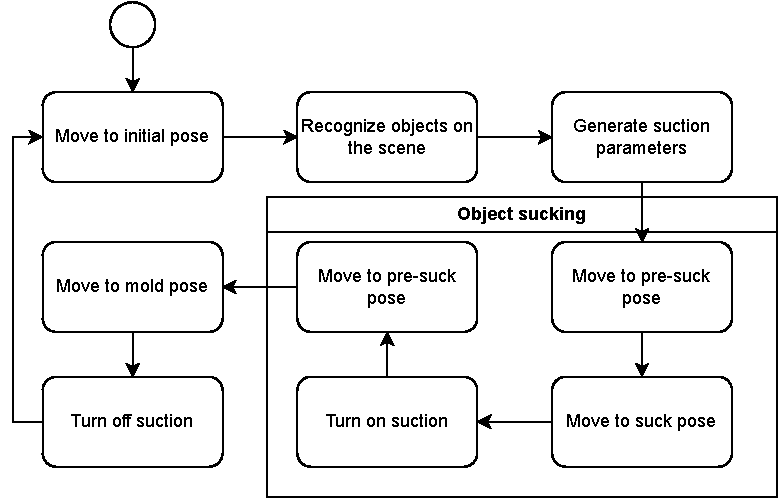
\includepdf[pagecommand=\subsection{FSM of the control subsystem}]{fsm_control_subsystem.pdf}




\end{document}
